% scusate, mi sono un po' rotto di continuare a cambiare lingua tra inglese e italiano, così ho deciso di riscrivere gli appunti per conto mio traducendo (con parecchi copia-incolla delle parti già in italiano)

\documentclass[a4page, 11pt]{article}

\usepackage{graphicx}
\graphicspath{ {./img/} }

\usepackage{hyperref} %clickable stuffs
\usepackage{mathtools}
\usepackage[margin=1.3in]{geometry}
\usepackage[utf8]{inputenc}
\usepackage[italian]{babel}
\usepackage[autostyle]{csquotes}
\MakeOuterQuote{"} %almost there, i removed `` everywhere to make it work better! D.
\usepackage{enumitem}
\usepackage[backend=biber]{biblatex}

\addbibresource{biblio.bib}



\title{Data Management}
\author{}
\date{}

\begin{document}
\maketitle

\tableofcontents
\newpage

\section{Modelli di dati.}
Il \textit{data modelling} è uno strumento per descrivere parte del mondo reale, permettendo di immagazzinare dati in un database ed effettuare interrogazioni sfruttando un linguaggio creato ad hoc.
Il linguaggio di interrogazione deve essere comprensibile sia alla macchina che all'uomo, espressivo, semplice, flessibile e, se possibile, deve seguire degli standard.
Il modello di dati più famoso è quello relazionale (rappresentato da SQL).

I modelli di dati seguono il Teorema di CAP, introdotto da Eric Brewer nel 2000:
\begin{itemize}
\item Consistency: tutti i nodi vedono gli stessi dati allo stesso istante;
\item Availability: ogni nodo deve rispondere alle richieste rivoltegli;
\item Partition Tolerance: il sistema funziona anche con dati frammentanti su una rete di calcolatori.
\end{itemize}
È impossibile per un modello soddisfare contemporaneamente tutte e tre le caratteristiche\cite{NoSQLDB}.
Il modello relazionale segue le leggi CA, mentre i modelli NoSQL sono CP o AP (dipende dal modello).
Si tende a preferire la disponibilità alla coerenza per ottenere dati non aggiornati piuttosto che messaggi di errore.


\subsection{SQL.}
Nato negli anni '70, il modello relazionale è ben sviluppato e conosciuto e gode di un'ottima reputazione: è stato lo standard \textit{de facto} per anni ed è ancora considerato il migliore per garantire l'integrità dei dati (permessa dal suo schema rigido).
Il modello relazionale segue quattro proprietà rappresentate dalla sigla ACID:
\begin{itemize}
\item Atomicity: l'operazione è \textit{atomica}, ovvero o avviene per intero (\texttt{COMMIT}) o restituisce un errore e il database ritorna alla forma iniziare (\texttt{ROLLBACK});
\item Consistency: i nuovi dati inseriti rispecchiano lo schema prestabilito (o l'operazione di inserimento fallisce);
\item Isolation: le singole operazioni non influiscono sulle altre; per fare questo il database costruisce una coda di esecuzione dei processi, così lo stato del database non muta durante l'esecuzione di una singola richiesta;
\item Durability: la persistenza del file è garantita (virtualmente a tempo indefinito) anche in caso di crash del sistema; per ottenere questo risultato sono utilizzati backup e log files.
\end{itemize}

Il modello relazionale tuttavia è fortemente influenzato dalla tecnologia degli anni in cui è nato: permette infatti di archiviare la maggior quantità di informazione occupando il minor spazio possibile su disco (allora gli hard disk erano costosi e ingombranti).
Nel tempo dunque si sono notati difetti nel modello:
\begin{itemize}[noitemsep]
\item un attributo può avere solo un tipo di valore;
\item SQL non è compatibile con i moderni linguaggi di programmazione ad oggetti;
\item la struttura del modello è molto rigida;
\item non permette loop nei dati;
\item la modifica di tabelle esistenti è difficile e dispendiosa.
\end{itemize}

Negli anni dunque si sono cercati modelli alternativi.
Nei RDBMS la performance (cioè la velocità di esecuzione) dipende da vari fattori:
\begin{itemize}
\item numero delle righe;
\item tipo di operazione;
\item algoritmo scelto;
\item struttura dei dati.
\end{itemize}

Inoltre il modello relazionale rende difficile scalare l'hardware: è stato pensato per poter girare su un'unica macchina fisica\footnote{Il modello \textit{NewSQL} proposto nel 2011 tenta di risolvere a questo inconveniente}.


\subsection{NoSQL.}
Per risolvere i problemi dei database relazionali, nasce un movimento informatico chiamato NoSQL (\textit{Not Only SQL}) che non rifiuta il modello ma propone approcci alternativi: i database NoSQL non hanno un modello prestabilito rendendo facile archiviare dati non strutturati e permettendo di aggiungere attributi senza modificare l'intero modello.
Mentre il modello relazionale si basa sull'assunzione del \textit{mondo chiuso}\footnote{\url{https://it.wikipedia.org/wiki/Ipotesi_del_mondo_chiuso}} (se il valore di verità non è noto, si considera la proposizione falsa), i modelli NoSQL adottano il modello del \textit{mondo aperto}\footnote{\url{https://it.wikipedia.org/wiki/Ipotesi_del_mondo_aperto}} secondo il quale non si può stabilire il valore di verità di cosa non è noto.

È possibile \textit{scalare} (\textit{scaling}) un DBMS potenziando l'hardware su cui è ospitato. Si distingue lo \textit{Scaling Up}, il potenziare la singola macchina, dallo \textit{Scaling out}, aggiungere macchine in una rete di calcolatori; quest ultimo caso è molto difficile da effettuare su un database di tipo relazionale. Il costo è un altro dei problemi: l'acquisto di macchine di una certa potenza è molto alto e non garantisce un aumento lineare delle prestazioni, che anzi scendono asintoticamente.

Opponendosi alla rigidità del modello relazionale, le proprietà dei database NoSQL non potevano che essere riassunte dall'acronimo BASE:
\begin{itemize}
\item Basic Availability: la consistenza può anche non essere garantita interamente, mostrando solamente una parte dei dati realmente disponibili (è il tipico caso di crash di un nodo che quindi non può trasmettere i dati al resto della rete);
\item Soft State: i dati possono avere schemi diversi (a differenza del modello relazionale);
\item Eventual Consistency: i sistemi NoSQL richiedono che, ad un certo punto, i dati convergano a uno stato consistente senza specificare quando; prima del raggiungimento della consistenza si possono avere valori non veritieri.
\end{itemize}

\begin{center}
\begin{tabular}{l|l}
ACID & BASE \\
\hline
Forte Coerenza & Coerenza debole \\
Poca disponibilità & Forte disponibilità \\
Difficilmente scalabile & Facilmente scalabile\\
Rigido & Flessibile \\
\end{tabular}
\end{center}

I modelli NoSQL si dividono in quattro macrocategorie\cite{NoSQLDB, GraphDB}:
\begin{enumerate}[noitemsep]
\item Document based (CouchDB, MongoDB): di solito salvati con file JSON, contenente un insieme ordinato di coppie \textless{}chiave - valore\textgreater{}; è facile ricercare dati in questo formato;
\item Graph based (Neo4J, FlockDB): sfrutta il concetto matematico di grafo per archiviare i dati come nodi ed esaltare i legami tra di essi costruendo archi; è difficile da scalare per quanto riguarda l'immagazzinamento (è difficile tagliare un grafo) ma è molto rapido nelle query.
\item Key Value (Dynamo, Voldemort, Rhino DHT): sono delle tabelle di coppie \textless{}chiave - valore\textgreater{} con chiavi che si riferiscono (o puntano) a un certo dato, è molto simile ai Document based.
\item Column family (Big Table, Cassandra): sono tabelle sparse e annidate contenenti coppie \textless{}chiave - valore\textgreater{}, sono in grado di salvare grandi quantità di dati.
\end{enumerate}

Costando di meno lo spazio di archiviazione, questi modelli non tentano di minimizzare lo spazio occupato su disco ma puntano a massimizzare le prestazioni nelle operazioni di R/W.
La ridondanza dei dati facilita questo compito pur aumentando notevolmente le dimensioni dei dati stessi: si sacrifica spazio di archiviazione a favore della velocità di lettura.
La semplicità del modello permette di archiviare un maggior numero di dati:
\begin{center}
	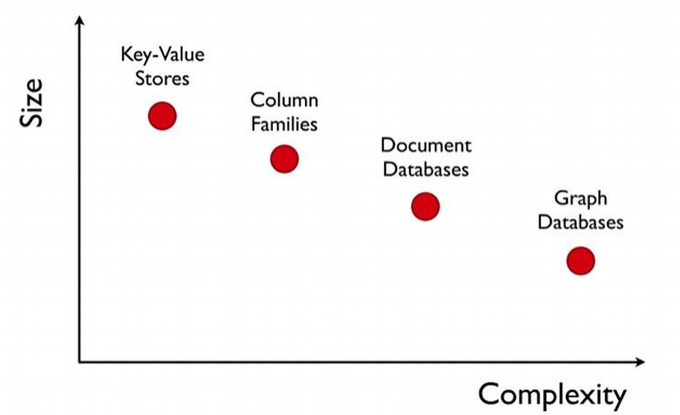
\includegraphics[scale=0.4]{IMAGE1.jpg}
\end{center}


\subsubsection{Document Based: MongoDB\cite{MongoDB, ScalingMongoDB}.}
MongoDB è, come già affermato, un sistema di gestione basato sui documenti (\textit{Document Based Management System}), in cui i dati sono archiviati in formato BSON (Binary JSON) e letti tramite indici. Mongo DB non prevedere operazioni di join. Cambiano i nomi delle entità rispetto al modello relazionale:
\begin{center}
  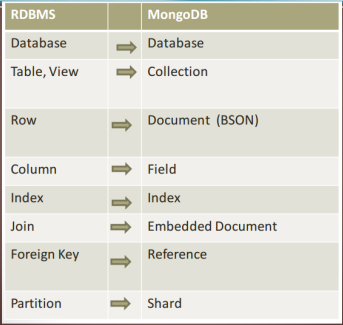
\includegraphics[scale=0.6]{IMAGE2.jpg}
\end{center}

Lavorando su una rete di calcolatori, MongoDB può impiegare un tempo considerevole a importare documenti da un database presistente; nel caso in cui si si voglia velocizzare il processo, si potrebbe decidere di apportare alcune modifiche:
\begin{itemize}[noitemsep]
\item disabilitare il riconoscimento dei dati, che è un segnale trasmesso tra processi di comunicazione, computer o dispositivi, per indicare il riconoscimento o la ricezione del messaggio, come parte di un protocollo di comunicazione;
\item disabilitare la scrittura su un file di tipo log che ha funzione di backup.
\end{itemize}
Bisogna stare molto attenti nel fare ciò, perché ogni ogni perdita non sarà registrata e di conseguenza sarà definitiva.
\newline

Per dataset di grandi dimensioni risulta molto utile l'utilizzo di indici: simili agli indici dei libri (o delle tabelle SQL), rappresentano un modo più veloce per recuperare informazioni.
L'uso di indici rallenta l'inserimento di nuovi dati (perché appunto devono essere indicizzati) ma velocizza notevolmente le ricerche. Il campo \texttt{\_id} è sempre indicizzato.
Senza un indice, MongoDB analizza a tappeto tutti i documenti (esattamente come SQL). Metaforicamente dovrebbe leggere ogni volta tutto il libro per recuperare l'informazione.
L'indicizzazione evita proprio questo problema (che aumenta con le dimensioni della \textit{collection}) organizzando il contenuto in una lista ordinata.
Dato che l'indicizzazione rallenta le modifiche, è buona norma utilizzare solamente un paio di indici per ogni collection; il limite di MongoDB è di 64 indici.
Il comando è il seguente:
\begin{verbatim}
db.<collection>.ensureIndex({
  <field1> : <sorting>,
  <field2> : <sorting> ...
});
\end{verbatim}
dove \texttt{<sorting>} assume il valore $+1$ per ordinamenti in ordine crescente e $-1$ per ordine decrescente. I campi \texttt{field} devono essere presenti in tutti i documenti della collection.

È possibile effettuare una sorta di \texttt{join} in MongoDB grazie all'algoritmo \textit{pipeline}\cite{NoSQLDB}, che però impiega più tempo del corrispettivo SQL.
Pipeline permette di eseguire operazioni di \texttt{\$match} e \texttt{\$group} su una collection così da eseguire una operazione su insiemi di risultati.
\begin{center}
  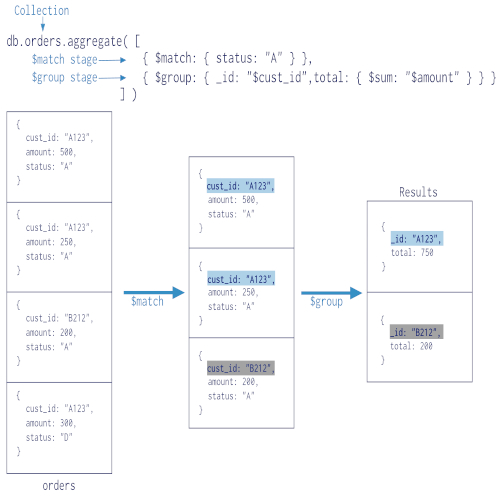
\includegraphics[scale=0.6]{mongodb-pipeline.jpg}
\end{center}

Per ragioni commerciali, MongoDB offre anche un'interfaccia SQL tramite il connettore BI (Business Intelligence): genera lo schema relazionale e lo usa per accedere ai dati.


\subsubsection{GraphDB: Neo4J\cite{GraphDB}.}
Un grafo è una collezione di nodi e archi, i quali rappresentano le relazioni tra i nodi stessi.
È facile modellare numerose realtà, come: social media, raccomandazioni, luoghi geografici, reti logistiche, grafici per le transazioni finanziarie (per il rilevamento delle frodi), master data management, bioinformatica, sistemi di autorizzazione e controllo degli accessi.
Il modello a grafo con etichette (\textit{labeled-property graph model}) ha le seguenti caratteristiche:
\begin{itemize}[noitemsep]
\item contiene \textit{nodi} e \textit{relazioni};
\item i nodi contengono \textit{proprietà} (coppie \textless{}chiave-valore\textgreater{});
\item i nodi possono essere etichettati con una o più \textit{etichette};
\item le relazioni sono nominali e direzionali, con un nodo d'inizio e uno di fine;
\item le relazioni, come i nodi, possono avere delle proprietà (e queste possono avere anche valori).
\end{itemize}
Le proprietà delle relazioni possono essere assegnate con un criterio \textit{fine-grained} o \textit{generic}. Considerando il caso della relazione \texttt{ADDRESS}, si può fare distinzione tra:
\begin{itemize}
\item fine-grained: \texttt{HOME\_ADDRESS}, \texttt{WORK\_ADDRESS} o \texttt{DELIVERY\_ADDRESS} (sono tutte etichette diverse);
\item generic: \texttt{ADDRESS:home}, \texttt{ADDRESS:work} o \texttt{ADDRESS:delivery} (l'etichetta è sempre \texttt{ADDRESS}, con un valore che ne indica il tipo).
\end{itemize}
Generalmente è preferito il secondo metodo per la minore complessità nello scrivere query (come ad esempio elencare tutti gli indirizzi di una data persona).

Un database a grafo può usare un motore di archiviazione nativamente a grafo o usare altri sistemi di archiviazione. Il primo ottimizza la gestione dei grafi, mentre il secondo archivia i dati in formato tabellare o tramite documenti per poi interrogare il database come se fosse un grafo.
Il metodo tabellare per esempio archivia le relazioni su una tabella relazionale che può essere interrogata tramite \textit{join bomb} (join con se stessa), tuttavia questo sistema degenera in fretta all'aumentare della distanza tra due nodi.

Il database a grafo risolve quindi il problema dei database relazionali (e di molti altri database NoSQL) a gestire le relazioni interne ai dati.
Infatti anche altri modelli NoSQL, indipendentemente dal modello adottato, soffrono perdite di prestazioni quando sono effettuate aggregazioni (soprattutto non indicizzati) dal momento che i collegamenti non sono nativi e manca il concetto di prossimità, presente invece nel grafo.
Si può tentare di risolvere il problema con dati annidati tra di loro ma la struttura del database risulterebbe eccessivamente complessa e non permetterebbe altre query.
Il DBA in base ai suoi bisogni (integrazione con altre applicazioni) può benissimo decidere di usare un database a grafo con una gestione dei dati non nativa senza che questo impatti sulla qualità del prodotto finale.
In un archivio nativo a grafo gli attributi, i nodi e i nodi referenziati sono memorizzati insieme per ottimizzare l'engine di processamento a grafo.

Per eseguire una query nel modello a grafo, il tempo di risposta non tipende strettamente dal numero totale di nodi (che rimane più o meno costante) perché la query viene processata nella porzione locale del grafo connessa al nodo base, mentre nei modelli relazionali e altri modelli NoSQL le prestazioni calano al aumentare dei dati (spesso in una maniera lineare).
Inoltre è possibile aggiungere altri nodi e relazioni senza disturbare il modello già esistente anche nel caso in cui i dati non abbiano la stessa struttura.
Il processing engine usa \textit{``index-free adjacency''} cioé i nodi connessi sono collegati fisicamente tra di loro, ciò velocizza il loro recupero da una query, ma questa velocità ha un prezzo: l'efficacia delle query che non sfruttano le proprietà del grafo viene peggiorata, ad esempio nel caso delle operazioni di R/W.   

Neo4j implementa un linguaggio Cypher, di tipo dichiartivo, che permette query al grafo usando una sitassi simile a SQL o SPARQL, ma comunque ottimizata per i grafi.
Cypher è facile da leggere e capire ed espressivo, pur rimanendo compatto.
Il linguaggio astrae il concetto di grafo permettendo all'autore di una query di indicare solamente cosa desidera tralasciando come. \newline
Neo4J utilizza in parallelo il linguaggio Gremlin, parte del framework Apache TinkerPop, che invece permette di esplicitare le modalità con cui deve essere svolta una richiesta al database.

\newpage
\printbibliography[title={Letture di approfondimento}]
\end{document}